\subsection{Trigonometrische Funktionen}
\subsubsection{Die Winkelfunktionen rechtwinkliger Dreiecke}
Grundlegend gibt es drei Winkelfunktionen, welche auf rechtwinklige Dreiecke angewandt werden k"onnen.\\
Zum einen w"are das der Sinus, dann der Kosinus und letztendlich der Tangens.\\
Die drei Seiten des Dreiecks werden als Hypotenuse (l"angste Seite des Dreiecks, -gegen"uber des rechten Winkels-), Ankathete (kurze Seite, welche am Winkel $\alpha$ anliegt), und Gegenkathete (Seite gegen"uber des Winkels $\alpha$) bezeichnet.
\begin{minipage}{7 cm}
\begin{enumerate}
\item $\sin(\alpha)=\frac{Gegekathete}{Hypotenuse}$
\item $\cos(\alpha)=\frac{Ankathete}{Hypotenuse}$
\item $\tan(\alpha)=\frac{sin(\alpha)}{\cos(\alpha)}= \frac{Gegenkathete}{Ankathete}$
\end{enumerate}
\end{minipage}
\begin{minipage}{6 cm}
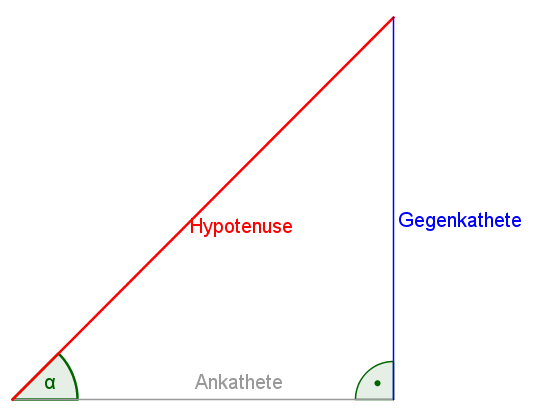
\includegraphics[width = 6 cm]{pictures/TrigonDreieck}
\end{minipage}

\subsubsection{Der Einheitskreis}
\begin{minipage}{9 cm}
Am besten sieht man die Eigenschaften der Winkelfunktionen bei der Betrachtung des\\ \textcolor{red}{Einheitskreises}.\\
Der Einheitskreis ist an sich nichts anderes als ein Kreis, mit Radius r = 1 LE und Kreismittelpunkt im Ursprung.\\
\end{minipage}
\begin{minipage}{4 cm}
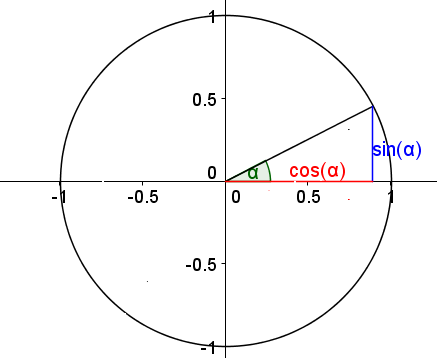
\includegraphics[width = 4 cm]{pictures/Einheitskreis}
\end{minipage}
Dabei ist die x-Koordinate des Punktes, am Ende der Hypotenuse des eingezeichneten Dreiecks, der Kosinuswert des Winkels Alpha und die y-Koordinate der Sinuswert.\\
Der Tangens ist die Steigung der Hypotenuse.


\subsubsection{Winkelma"s und Bogenma"s}
Bisher haben wir immer mit Winkelma"sen gerechnet, wie zum Beispiel $45^\circ$. Neben dieser M"oglichkeit, Winkel auszudr"ucken, gibt es auch noch das Bogenma"s.\\
Definition: Das Bogenma"s ist die L"ange des Kreisbogens mit dem Radius r = 1 unter einem bestimmten Winkel.\\
Wie ein Winkelwert mit $^\circ$ gekennzeichnet wird, so kennzeichnet man das Bogenma"s mit dem W"ortchen "'rad"'.\\
An den meisten "'h"oheren"' Schulen wird das Bogenma"s bevorzugt.
\subsubsection{Graphische Darstellung der Winkelfunktionen}
Stellt man die Winkelfunktionen graphisch dar, so bekommt man folgende Zeichnungen.\vspace{0.5 cm}\\
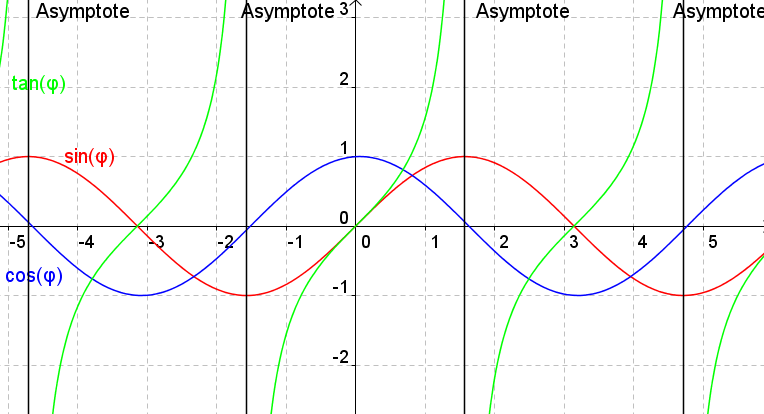
\includegraphics[width = 13 cm, height = 5 cm]{pictures/Winkelfunktionen}
\subsubsection{Nullstellen, Asymptoten und Symmetrie}
Alle Winkelfunktionen sind periodisch. Deshalb treten auch ihre Nullstellen in gleichbleibenden Abst"anden auf.
\begin{itemize}
\item Sinusfunktion: $x+n*\pi rad$ , welche sich mit den Nullstellen der Tangesnfunktion decken
\item Kosinusfunktion: $(0,5+n)*\pi rad$
\end{itemize}
Des Weiteren besitzt die Tangensfunktion eine periodisch auftretende senkrechte Asymptote an den Nullstellen des Kosinus.\\
Betrachtet man die Graphen im Hinblick auf ihre Symmetrie bez"uglich des Koordinatensystems, stellt man fest, dass die Sinus- und Tangesnsfunktion punktsymmetrisch zum Ursprung (ungerade) und die Kosinusfunktion achsensymmetriesch zur y-Achse (gerade) ist.